\documentclass[14pt]{article}
\usepackage{polski}
\usepackage[utf8]{inputenc}
\usepackage{amsmath}
\usepackage{amsfonts}
\usepackage{tabto,lipsum}
\usepackage{xcolor}
\usepackage{shadowtext}
\usepackage{hyperref}
\hypersetup{%
  colorlinks=false,% hyperlinks will be black
  linkbordercolor=red,% hyperlink borders will be red
  pdfborderstyle={/S/U/W 1}% border style will be underline of width 1pt
}
\usepackage[margin=3cm]{geometry}

\usepackage{tikz}
\usetikzlibrary{arrows}

\tikzset{
  treenode/.style = {row sep=10pt,align=center, inner sep=0pt, text centered,
    font=\sffamily},
  arn_n/.style = {treenode, circle, white, font=\sffamily\bfseries, draw=black,
    fill=black, text width=1.5em},% arbre rouge noir, noeud noir
  arn_r/.style = {treenode, circle, red, draw=red,
    text width=1.5em, very thick},% arbre rouge noir, noeud rouge
  arn_x/.style = {treenode, rectangle, draw=black,
    minimum width=0.5em, minimum height=0.5em}% arbre rouge noir, nil
}

\linespread{1.3}

\title{Lista 4}
\author{Zadanie 12}
\date{---------------------}



\begin{document}

\maketitle

\section{RB-Tree}
Dodajemy kolejno wartości $41, 38, 31, 12, 19, 8$ do drzewa czerwono-czarnego.

\subsection{}
Dodajemy $41$.

\begin{center}

\begin{tikzpicture}[->,>=stealth',level/.style={sibling distance = 5cm/#1,
  level distance = 1.5cm}]
\node [arn_r] {41}
;
\end{tikzpicture}
\end{center}

\subsection{}

Tutaj w zależności od konwencji można zamienić kolor w celu zachowania koloru czarnego węzła początkowego. My będziemy się trzymać tej konwencji czarnego \textit{roota}.

\begin{center}

\begin{tikzpicture}[->,>=stealth',level/.style={sibling distance = 5cm/#1,
  level distance = 1.5cm}]
\node [arn_n] {41}
;
\end{tikzpicture}
\end{center}

\subsection{}
Wstawiamy $38$.

\begin{center}
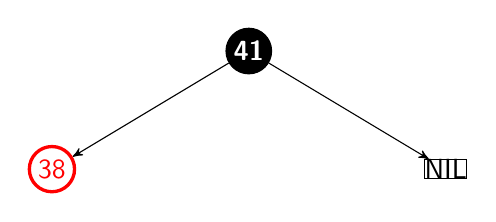
\begin{tikzpicture}[->,>=stealth',level/.style={sibling distance = 5cm/#1,
  level distance = 1.5cm}]
\node [arn_n] {41}
    child{ node [arn_r] {38}}
    child{ node [arn_x] {NIL}}
;
\end{tikzpicture}
\end{center}

\subsection{}
Wstawiamy $31$ i od razu zmieniamy kolor na czarny.

\begin{center}
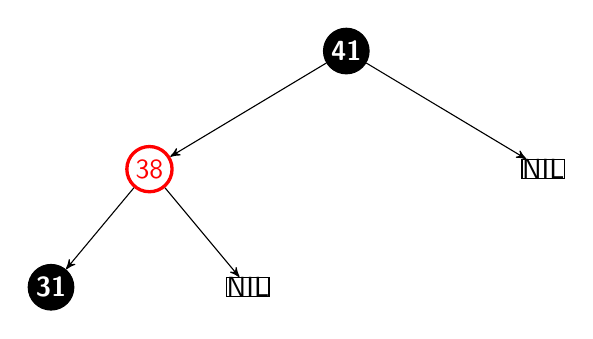
\begin{tikzpicture}[->,>=stealth',level/.style={sibling distance = 5cm/#1,
  level distance = 1.5cm}]
\node [arn_n] {41}
    child{ node [arn_r] {38}
        child{ node [arn_n] {31}}
        child{ node [arn_x] {NIL}}
    }
    child{ node [arn_x] {NIL}}
;
\end{tikzpicture}
\end{center}

Musimy dokonać rotacji żeby zachować parametr odnoszący się do czarnej wysokości drzewa.
Aktualnie droga $41 \rightarrow 38 \rightarrow 31 \rightarrow \text{NIL}$ zawiera dwa czarne węzły nie licząc \textit{roota}.

\begin{center}
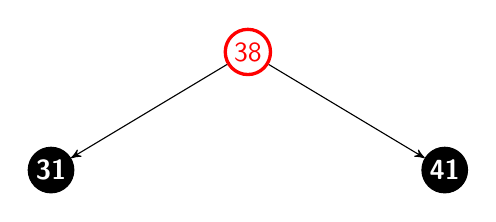
\begin{tikzpicture}[->,>=stealth',level/.style={sibling distance = 5cm/#1,
  level distance = 1.5cm}]
\node [arn_r] {38}
    child{ node [arn_n] {31}}
    child{ node [arn_n] {41}}
;
\end{tikzpicture}
\end{center}

Zamieniamy kolory, żeby węzeł początkowy był czarny.

\begin{center}
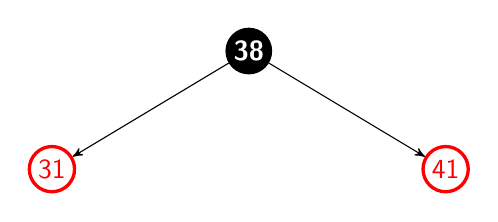
\begin{tikzpicture}[->,>=stealth',level/.style={sibling distance = 5cm/#1,
  level distance = 1.5cm}]
\node [arn_n] {38}
    child{ node [arn_r] {31}}
    child{ node [arn_r] {41}}
;
\end{tikzpicture}
\end{center}

\subsection{}

Wstawiamy $12$.

\begin{center}
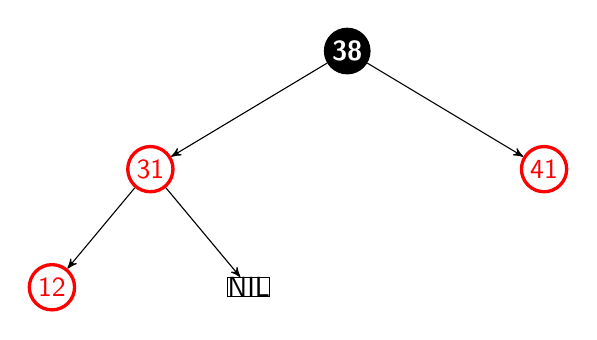
\begin{tikzpicture}[->,>=stealth',level/.style={sibling distance = 5cm/#1,
  level distance = 1.5cm}]
\node [arn_n] {38}
    child{ node [arn_r] {31}
        child{ node [arn_r] {12}}
        child{ node [arn_x] {NIL}}
    }
    child{ node [arn_r] {41}}
;
\end{tikzpicture}
\end{center}

Zmieniamy kolor $12$ żeby zachować zasadę co do potomków węzłów czerwonych. Jednocześnie zapewniamy, że czarna wysokość drzewa się zgadza. Idąc od \textit{roota} za każdym razem czarna wysokość jest taka sama, nieważne jaką ścieżkę wybierzemy.

\begin{center}
  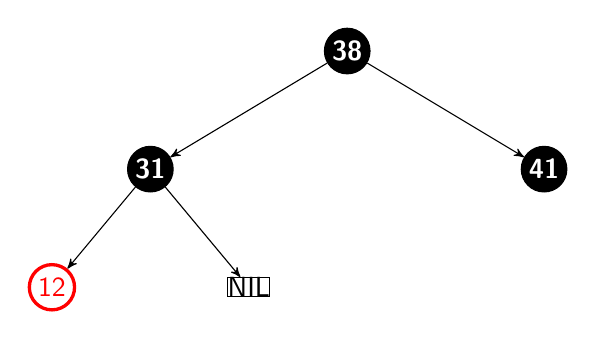
\begin{tikzpicture}[->,>=stealth',level/.style={sibling distance = 5cm/#1,
    level distance = 1.5cm}]
  \node [arn_n] {38}
      child{ node [arn_n] {31}
          child{ node [arn_r] {12}}
          child{ node [arn_x] {NIL}}
      }
      child{ node [arn_n] {41}}
  ;
  \end{tikzpicture}
  \end{center}

\subsection{}

Wstawiamy $19$.

\begin{center}
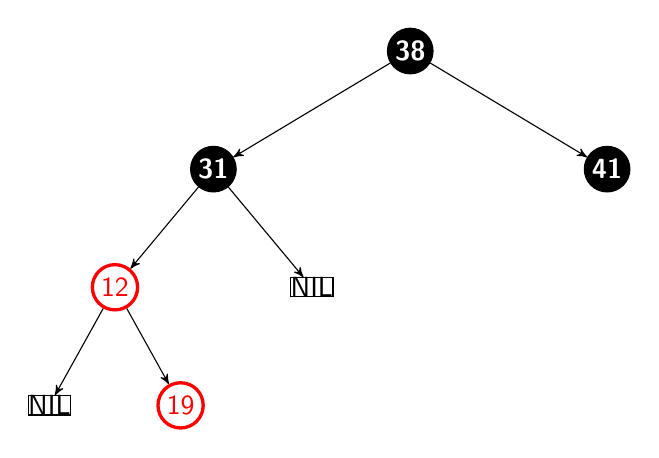
\begin{tikzpicture}[->,>=stealth',level/.style={sibling distance = 5cm/#1,
  level distance = 1.5cm}]
\node [arn_n] {38}
    child{ node [arn_n] {31}
        child{ node [arn_r] {12}
            child{ node [arn_x] {NIL}}
            child{ node [arn_r] {19}}
        }
        child{ node [arn_x] {NIL}}
    }
    child{ node [arn_n] {41}}
;
\end{tikzpicture}
\end{center}

Dokonujemy rotacji $12$ w lewą stronę.

\begin{center}
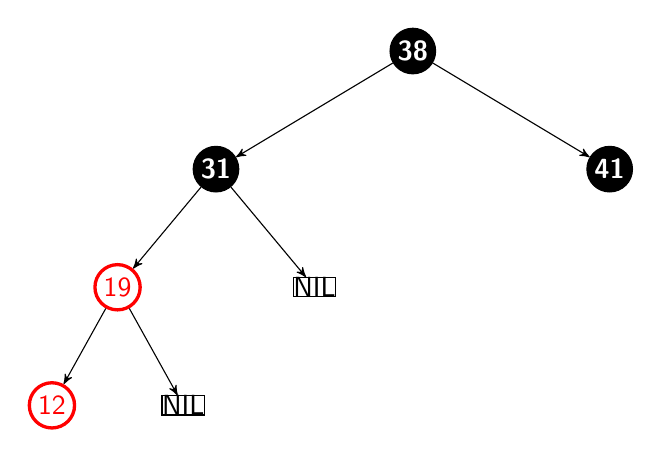
\begin{tikzpicture}[->,>=stealth',level/.style={sibling distance = 5cm/#1,
  level distance = 1.5cm}]
\node [arn_n] {38}
    child{ node [arn_n] {31}
        child{ node [arn_r] {19}
            child{ node [arn_r] {12}}
            child{ node [arn_x] {NIL}}
        }
        child{ node [arn_x] {NIL}}
    }
    child{ node [arn_n] {41}}
;
\end{tikzpicture}
\end{center}

Dokonujemy rotacji $31$ w prawą stronę.

\begin{center}
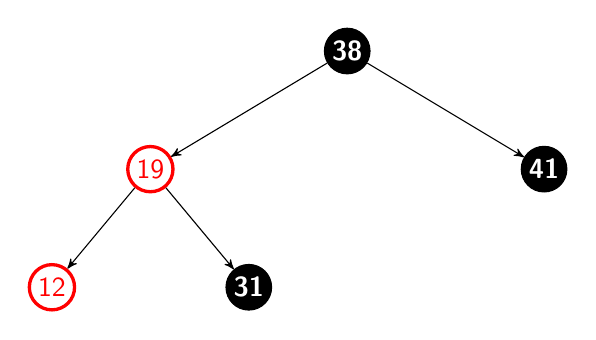
\begin{tikzpicture}[->,>=stealth',level/.style={sibling distance = 5cm/#1,
  level distance = 1.5cm}]
\node [arn_n] {38}
    child{ node [arn_r] {19}
        child{ node [arn_r] {12}
        }
        child{ node [arn_n] {31}}
    }
    child{ node [arn_n] {41}}
;
\end{tikzpicture}
\end{center}

Zmieniamy kolory $19$ i $31$ w celu zachowania odpowiedniej czarnej wysokości.

\begin{center}
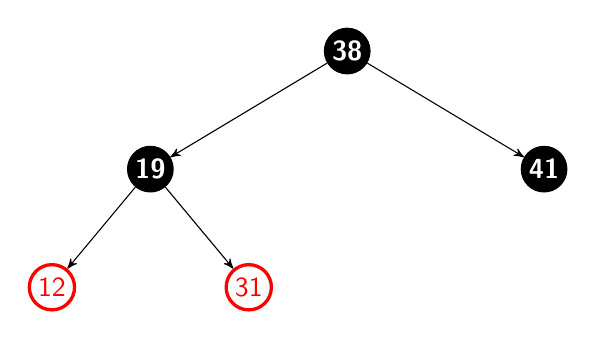
\begin{tikzpicture}[->,>=stealth',level/.style={sibling distance = 5cm/#1,
  level distance = 1.5cm}]
\node [arn_n] {38}
    child{ node [arn_n] {19}
        child{ node [arn_r] {12}
        }
        child{ node [arn_r] {31}}
    }
    child{ node [arn_n] {41}}
;
\end{tikzpicture}
\end{center}

\subsection{}

Wstawiamy $8$.


\begin{center}
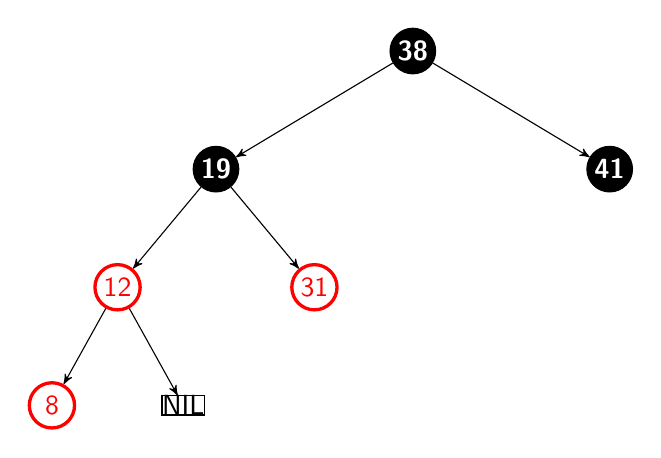
\begin{tikzpicture}[->,>=stealth',level/.style={sibling distance = 5cm/#1,
  level distance = 1.5cm}]
\node [arn_n] {38}
    child{ node [arn_n] {19}
        child{ node [arn_r] {12}
            child{ node [arn_r] {8}}
            child{ node [arn_x] {NIL}}
        }
        child{ node [arn_r] {31}}
    }
    child{ node [arn_n] {41}}
;
\end{tikzpicture}
\end{center}

W tym przypadku wystarczy zmienić kolory poziomów $12,31$ oraz $19$.

\begin{center}
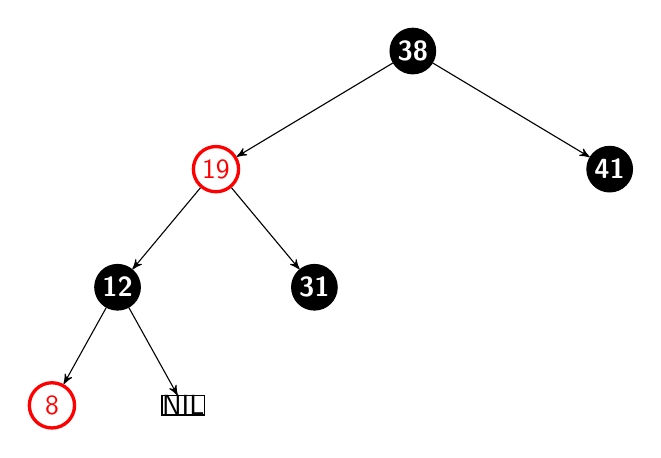
\begin{tikzpicture}[->,>=stealth',level/.style={sibling distance = 5cm/#1,
  level distance = 1.5cm}]
\node [arn_n] {38}
    child{ node [arn_r] {19}
        child{ node [arn_n] {12}
            child{ node [arn_r] {8}}
            child{ node [arn_x] {NIL}}
        }
        child{ node [arn_n] {31}}
    }
    child{ node [arn_n] {41}}
;
\end{tikzpicture}
\end{center}

Nasze końcowe RB-Tree spełnia wszystkie warunki:

\begin{itemize}
  \item Każdy liść przechowujący wartość $\mathrm{NIL}$ jest czarny
  \item Jeśli węzeł jest czerwony, to obaj jego potomkowie są czarni
  \item Każda prosta ścieżka z ustalonego węzła do liścia ma tyle samo czarnych węzłów (zachowana jest czarna wysokość drzewa)
\end{itemize}

\section{Binary Search Tree (BST)}
Dodajemy kolejno wartości $41, 38, 31, 12, 19, 8$ do drzewa BST.

\begin{center}

\begin{tikzpicture}[->,>=stealth',level/.style={sibling distance = 5cm/#1,
  level distance = 1.5cm}]
\node [arn_n] {41}
;
\end{tikzpicture}
\end{center}

\begin{center}
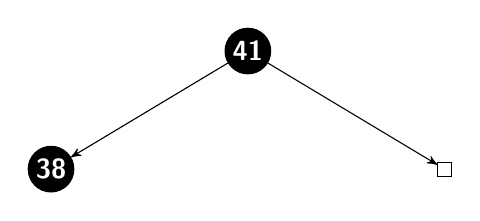
\begin{tikzpicture}[->,>=stealth',level/.style={sibling distance = 5cm/#1,
  level distance = 1.5cm}]
\node [arn_n] {41}
  child{ node [arn_n] {38} }
  child{ node [arn_x] {}}
;
\end{tikzpicture}
\end{center}

\begin{center}
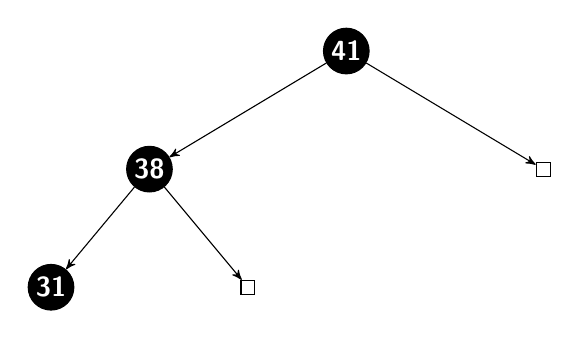
\begin{tikzpicture}[->,>=stealth',level/.style={sibling distance = 5cm/#1,
  level distance = 1.5cm}]
\node [arn_n] {41}
  child{ node [arn_n] {38}
    child{node [arn_n] {31}}
    child{ node [arn_x] {}}
  }
  child{ node [arn_x] {}}
;
\end{tikzpicture}
\end{center}

\begin{center}
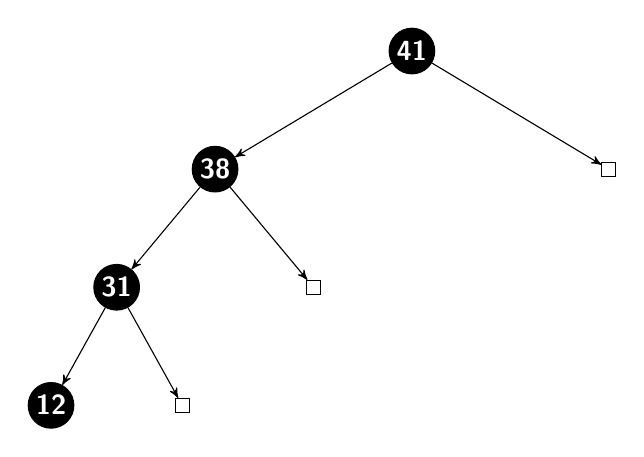
\begin{tikzpicture}[->,>=stealth',level/.style={sibling distance = 5cm/#1,
  level distance = 1.5cm}]
\node [arn_n] {41}
  child{ node [arn_n] {38}
    child{node [arn_n] {31}
      child{ node [arn_n] {12}}
      child{ node [arn_x] {}}
    }
    child{ node [arn_x] {}}
  }
  child{ node [arn_x] {}}
;
\end{tikzpicture}
\end{center}

\begin{center}
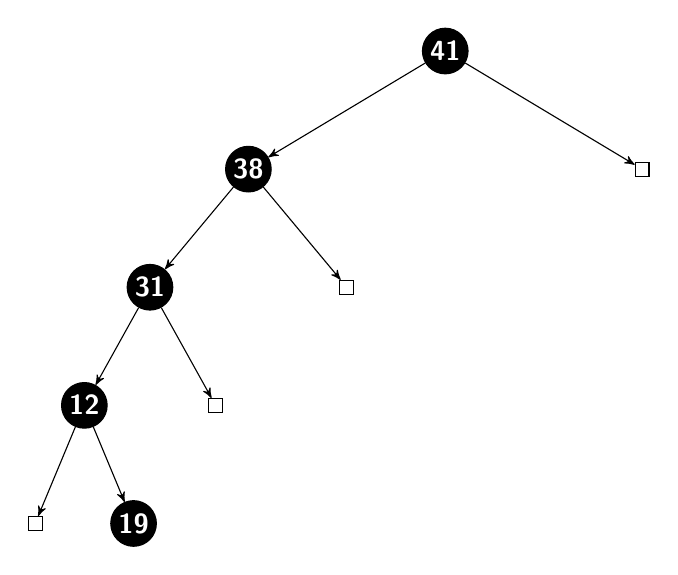
\begin{tikzpicture}[->,>=stealth',level/.style={sibling distance = 5cm/#1,
  level distance = 1.5cm}]
\node [arn_n] {41}
  child{ node [arn_n] {38}
    child{node [arn_n] {31}
      child{ node [arn_n] {12}
        child{ node [arn_x] {}}
        child{ node [arn_n] {19}}
      }
      child{ node [arn_x] {}}
    }
    child{ node [arn_x] {}}
  }
  child{ node [arn_x] {}}
;
\end{tikzpicture}
\end{center}

\begin{center}
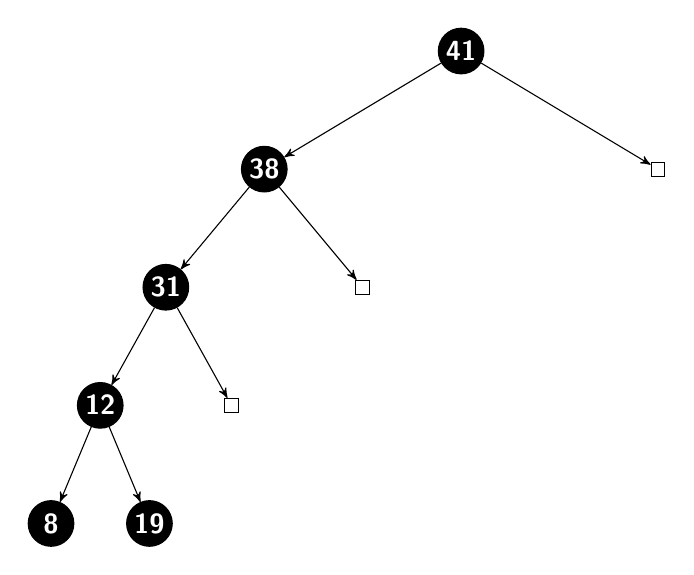
\begin{tikzpicture}[->,>=stealth',level/.style={sibling distance = 5cm/#1,
  level distance = 1.5cm}]
\node [arn_n] {41}
  child{ node [arn_n] {38}
    child{node [arn_n] {31}
      child{ node [arn_n] {12}
        child{ node [arn_n] {8}}
        child{ node [arn_n] {19}}
      }
      child{ node [arn_x] {}}
    }
    child{ node [arn_x] {}}
  }
  child{ node [arn_x] {}}
;
\end{tikzpicture}
\end{center}

\section{Wnioski}

Dzięki rygorystycznym zasadom, które obarczone są drzewa czerwonoczarne mamy tam znacznie lepszy balans elementów. Nawet jeśli dodajemy bardzo dużo elementów które są mniejsze niż ten co był na początku wysokość drzewa nie jest tak duża jak to jest w przypadku BST.

\end{document}
